\documentclass[conference]{IEEEtran}
\IEEEoverridecommandlockouts
% The preceding line is only needed to identify funding in the first footnote. If that is unneeded, please comment it out.
\include{../solutions}
\usepackage{cite}
\usepackage{amsmath,amssymb,amsfonts}
% \usepackage{algorithmic}
\usepackage{graphicx}
\usepackage{textcomp}
\usepackage{xcolor}
\usepackage{tabularx}
% \usepackage{hyperref}

\def\BibTeX{{\rm B\kern-.05em{\sc i\kern-.025em b}\kern-.08em
    T\kern-.1667em\lower.7ex\hbox{E}\kern-.125emX}}

\title{\LARGE{Radiogenomic Prediction of Breast Cancer Subtypes \\ Using the TCGA Dataset}}

\author{
    \begin{tabular}{c}
        \begin{tabular}{cc}
            \begin{tabular}{c} 
                \IEEEauthorblockN{Lucas Fayolle} \\
                \vspace{-8mm}
                \IEEEauthorblockA{\textit{lfayoll@etsinf.upv.es}}
            \end{tabular} &
            \begin{tabular}{c} 
                \vspace{-4.5mm}
                \IEEEauthorblockN{Jose Valero Sanchis} \\
                \vspace{-8mm}
                \IEEEauthorblockA{\textit{jvalsan@etsinf.upv.es}}
            \end{tabular}
        \end{tabular}
    \end{tabular}
}

\begin{document}

\maketitle

\begin{abstract}
Lorem ipsum dolor sit amet, consectetur adipiscing elit. Sed porta, ante at finibus egestas, neque neque lacinia ipsum, nec accumsan turpis mauris in est. Sed mollis consectetur felis, id fringilla lacus efficitur id. Maecenas iaculis mattis lacus, eget faucibus est maximus in. Pellentesque pulvinar tortor neque, in rhoncus lorem consequat ac. Ut varius urna et lorem laoreet, lacinia venenatis lacus elementum. In vel ante eget diam facilisis consequat vitae eu mauris. 
\end{abstract}

\begin{IEEEkeywords}
Mathematical Optimization, ...
\end{IEEEkeywords}

%%%%%%%%%%%%%%%%%%%%%%%%%%%%%%%%%%%%%%%%%%%%%%%%%%%%%%%%%%%%%%%%%%%%%%%%%%%%%%%
%                                                                                          INTRODUCTION                                                                                                                   %
%%%%%%%%%%%%%%%%%%%%%%%%%%%%%%%%%%%%%%%%%%%%%%%%%%%%%%%%%%%%%%%%%%%%%%%%%%%%%%%

\section{Introduction}

\subsection{Background and motivation}

Breast cancer is one of the most common cancers worldwide and a leading cause of mortality among women. Molecular profiling has identified subtypes such as Luminal A, Luminal B, HER2-enriched, and Basal-like, which are essential for guiding personalized treatments \cite{b1}. However, determining these subtypes often requires invasive procedures, such as biopsies and genomic assays, which can be costly and time-consuming.

Radiomics offers a non-invasive approach by extracting quantitative features from MRI images that can capture tumor phenotypic traits linked to molecular profiles. Integrating radiomic features with clinical and genomic data can enhance machine learning models for breast cancer subtype prediction, supporting precision oncology workflows. \cite{b2}

This project aims to develop a classifier that predicts molecular subtypes based on MRI-derived radiomic features and evaluates the impact of incorporating clinical and genomic data to improve performance.

\subsection{Project objectives}

The primary objective of this project is to develop a machine learning classifier capable of predicting the molecular subtypes of breast cancer (Luminal A, Luminal B, HER2-enriched, Basal-like) using radiomic features extracted from MRI images.

To achieve this, the following specific objectives are proposed:

\begin{itemize}
	\item \textbf{Utilization of the provided radiomic features}. A preprocessing pipeline will be applied to the radiomic data provided, incorporating variance filtering and feature selection methods, such as Boruta, to refine the input features. Once processed, the machine learning models will be trained and evaluated using relevant performance metrics to assess their predictive accuracy.

	\item \textbf{Incorporation of clinical data}. Clinical variables, such as age and tumor stage, will be integrated into the dataset. Models trained with this comprehensive feature set will be compared to previous models to evaluate the impact of clinical data on predictive performance.	

	\item \textbf{Integration of multigenic assay data}. Multigenic assay scores will be analyzed for correlations with radiomic features and added as predictors. Models will be trained with the extended dataset, and their performance will be assessed to determine if genomic data enhances prediction.
\end{itemize}

\subsection{Report structure}

This report is organized into five main sections. The Introduction presents the background, motivation, and objectives of the study. The Methodology describes the datasets used, the data preprocessing steps, and the exploratory data analysis, followed by the feature selection. The Model development section explains the different machine learning models created and the evaluation metrics used to assess their performance. The Results and discussion section compares the models' performance and analyzes the impact of incorporating clinical and genomic data. Finally, the Conclusions summarize the key findings, discuss limitations, and propose future work.

%%%%%%%%%%%%%%%%%%%%%%%%%%%%%%%%%%%%%%%%%%%%%%%%%%%%%%%%%%%%%%%%%%%%%%%%%%%%%%%
%                                                                                              Methodology                                                                                                                   %
%%%%%%%%%%%%%%%%%%%%%%%%%%%%%%%%%%%%%%%%%%%%%%%%%%%%%%%%%%%%%%%%%%%%%%%%%%%%%%%

\section{Methodology}

\subsection{Description of datasets}


The data used in this project was obtained from the TCGA Breast Radiogenomics collection available in \cite{b3}. Among other files, such as the original MRI images and their corresponding tumor segmentations (as shown in Figure \ref{fig:mri_example}, illustrating the type of imaging data from which radiomic features are extracted for analysis), the dataset includes three types of data sources: radiomic features, multigenic assay results, and clinical data:

\begin{itemize}
	\item \textbf{Quantitative Radiomic Features}.  This dataset includes 41 quantitative features derived from MRI images, which describe different aspects of the tumor, such 		as shape, texture, and signal enhancement dynamics.

	\item \textbf{MammaPrint, Oncotype DX, and PAM50 multi-gene assays}. This dataset provides genomic scores associated with breast cancer prognosis and subtype 			classification. The variable \textbf{Pam50.Call} serves as the target variable, indicating the molecular subtype for each sample.

	\item \textbf{Clinical data}. This dataset contains information on patient demographics, tumor characteristics, and treatment-related variables

\end{itemize}

\begin{figure}
    \centering
    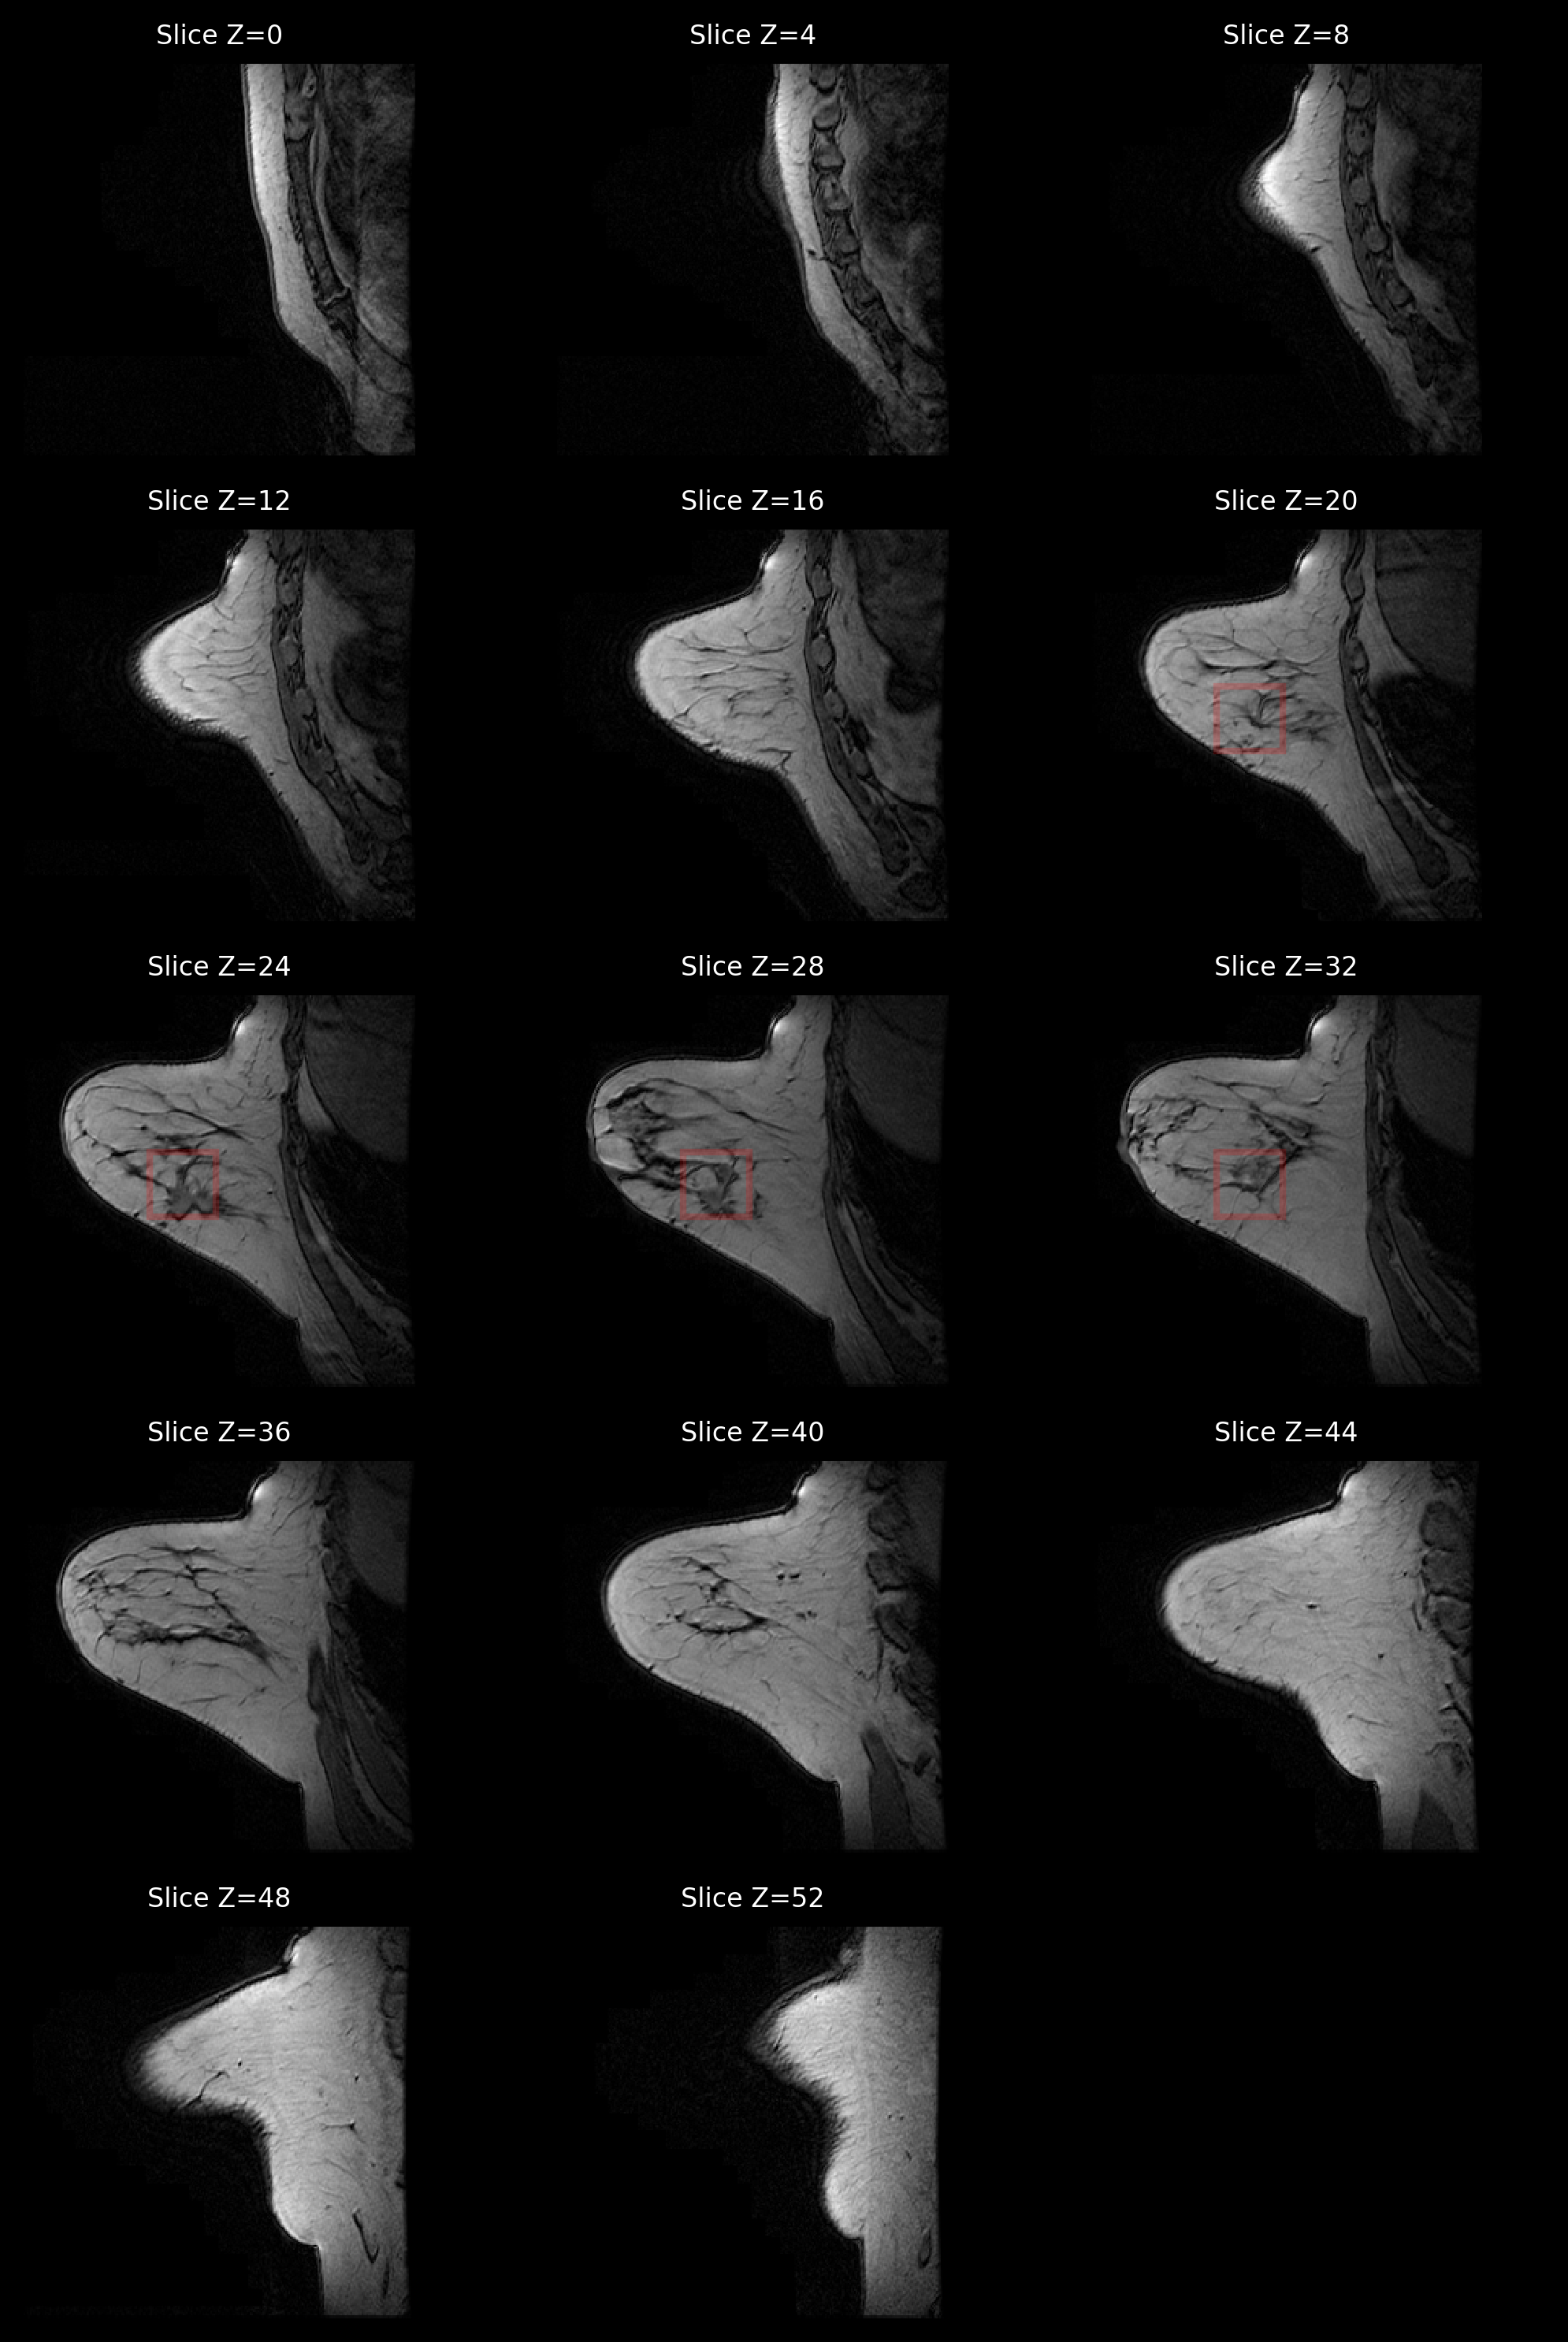
\includegraphics[width=0.45\textwidth]{images/mri_example.png}
    \caption{Example MRI scan with corresponding tumor segmentation}
    \label{fig:mri_example}
\end{figure}

\subsection{Data preprocessing}

The data preprocessing phase ensures that the dataset is consistent and focused on the relevant classification task by selecting complete instances and excluding irrelevant categories.

\subsubsection{Identification of complete instances}

In this step, we ensure that only instances with complete information across all datasets—radiomic features, multigenic assay results, and clinical data—are included. This guarantees that the training and evaluation of machine learning models are performed consistently with the same set of data points, regardless of the features being tested.

The approach involves checking for the presence of a common identifier (CLID) across the three datasets. Instances that do not have corresponding entries in the radiomic, multigenic, or clinical datasets are excluded.

As a result, a new dataset containing only the complete instances is created, ensuring uniformity in the data used across all experiments.

\subsubsection{Removal of the "normal" category}

In this step, instances labeled as "Normal" in the Pam50.Call variable are excluded from the dataset. The rationale behind this decision is that the focus of the project is to differentiate between molecular subtypes of breast cancer, not to distinguish between healthy and cancerous tissue. Including "Normal" as a class would introduce a category that lacks clinical relevance for the subtype prediction task, as "Normal" does not correspond to a specific cancer phenotype.

\vspace{5mm}

After this preprocessing, from the 84 cases present in the original dataset, 76 instances remain for analysis in this project. The distribution of the target variable in these instances is shown in Figure \ref{fig:pam_distr}.

\begin{figure}
    \centering
    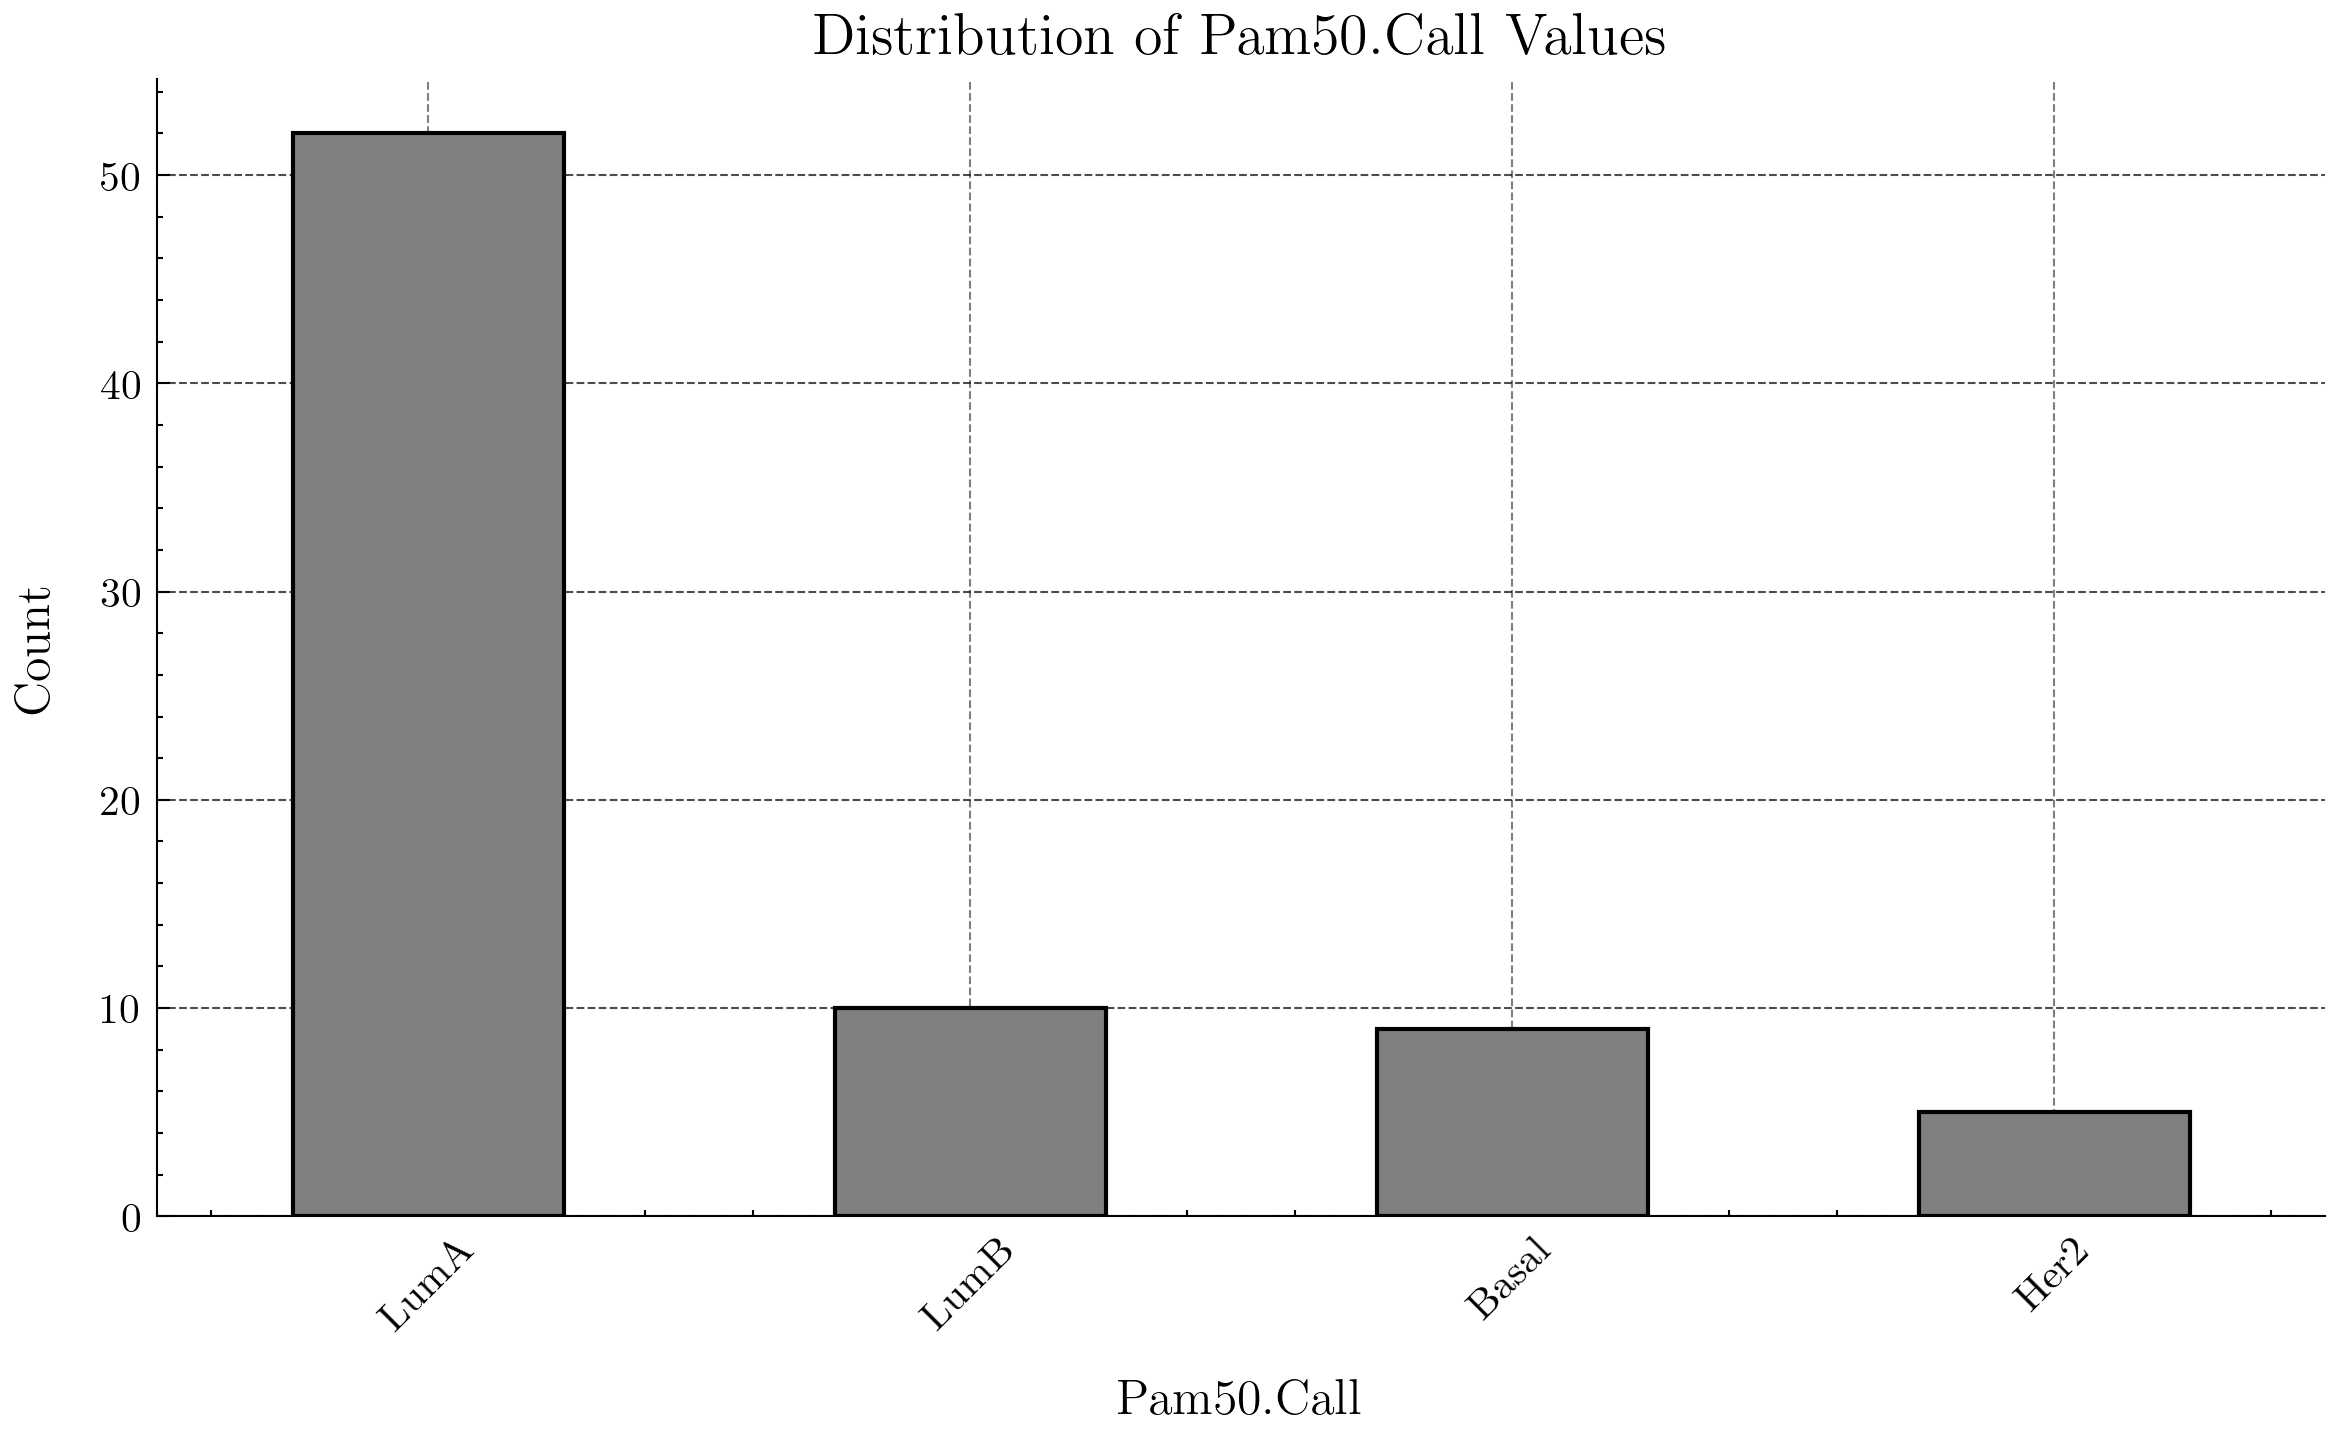
\includegraphics[width=0.5\textwidth]{images/pam_distr.png}
    \caption{Distribution of \texttt{Pam50.Call} values}
    \label{fig:pam_distr}
\end{figure}

As shown in Figure \ref{fig:pam_distr}, there is a significant class imbalance, with the Luminal A subtype being highly overrepresented compared to the other classes. This imbalance must be taken into account when selecting the evaluation metrics for the model. Additionally, as will be discussed later, undersampling and oversampling techniques will be applied to address this issue and improve the model’s robustness.

\subsection{Exploratory data analysis (EDA) and feature selection} (QUIZA DEJAR SOLO LA PARTE DE FEATURE SELECTION)

The exploratory data analysis (EDA) provides insights into the clinical data and multigenic assay scores, helping to understand their distribution, correlations, and relevance to the target variable. In addition to statistical findings, medical considerations are taken into account to ensure that the selected variables are not only informative but also clinically meaningful for inclusion in the model.

\subsubsection{Clinical data}

The clinical variables included in the model are the patient's age at the time of diagnosis, the cancer's overall stage and tumor size, the number of lymph nodes affected, and the status of estrogen and progesterone receptors. Their selection is based on both statistical  (METER QUIZA ANEXO) findings and clinical relevance:

\begin{itemize}
    \item \textbf{Age at diagnosis}. A key prognostic factor, as younger patients often have more aggressive tumors, while older patients may present less aggressive subtypes.
    \item \textbf{Cancer stage and tumor size}. These variables describe the extent of disease progression and are crucial for predicting molecular subtypes.
    \item \textbf{Number of affected lymph nodes}.  Indicates metastatic spread and reflects the severity of the disease.
    \item \textbf{Hormone receptor status (estrogen and progesterone)}. These statuses are essential for distinguishing Luminal subtypes. However, due to their high correlation with the target variable, a model was also built without them to avoid redundancy.
\end{itemize}

The HER2 receptor status based on immunohistochemistry results was excluded due to a high proportion of missing values, despite its relevance to the HER2-enriched subtype.

\subsubsection{Multigenic assay scores}

The following multigenic assay variables were selected based on their relevance to tumor biology and their ability to complement the radiomic and clinical data:

\begin{itemize}
    \item \textbf{GHI\_RS Score}. This continuous score, derived from the Oncotype DX assay, measures the risk of recurrence based on gene expression related to tumor growth and proliferation.
    \item \textbf{Correlation with good outcome signature}. This variable represents how strongly the sample correlates with a favorable prognosis gene profile from the MammaPrint assay. It enriches the model by offering complementary insights into the tumor's behavior and long-term prognosis.
    \item \textbf{Proliferation-related gene expression}. This variable captures the average expression of a set of genes associated with cell proliferation, a key marker of tumor aggressiveness. While not directly predictive of molecular subtype, it is particularly informative for identifying more aggressive subtypes, such as Basal-like or HER2-enriched.
\end{itemize}

%%%%%%%%%%%%%%%%%%%%%%%%%%%%%%%%%%%%%%%%%%%%%%%%%%%%%%%%%%%%%%%%%%%%%%%%%%%%%%%
%                                                                                              Model development                                                                                                        %
%%%%%%%%%%%%%%%%%%%%%%%%%%%%%%%%%%%%%%%%%%%%%%%%%%%%%%%%%%%%%%%%%%%%%%%%%%%%%%%

\section{Model development}

\subsection{Model creation}

% Explicar como se ha creado cada modelo (extenderse sobretodo en el primero, en el resto unicamente es añadir variables)

\subsubsection{Radiomic features-based model}

\subsubsection{Radiomic model with clinical data}

\subsubsection{Radiomic model with multigenic assays}

\subsection{Evaluation metrics used}

% F1-macro por el desbalanceo de clases

\subsection{Model performance results}

% Además, de los modelos "explicados", incluir tambien los resultados de clinical data y multigentic assays sin radiomica, para ver si radiomica aporta algo o no.


%%%%%%%%%%%%%%%%%%%%%%%%%%%%%%%%%%%%%%%%%%%%%%%%%%%%%%%%%%%%%%%%%%%%%%%%%%%%%%%
%                                                                                              Results and discussion                                                                                                      %
%%%%%%%%%%%%%%%%%%%%%%%%%%%%%%%%%%%%%%%%%%%%%%%%%%%%%%%%%%%%%%%%%%%%%%%%%%%%%%%

\section{Results and discussion}

\subsection{Comparison of model performance}

\subsection{Impact of clinical data inclusion}

\subsection{Impact of multigenic assays on prediction}


%%%%%%%%%%%%%%%%%%%%%%%%%%%%%%%%%%%%%%%%%%%%%%%%%%%%%%%%%%%%%%%%%%%%%%%%%%%%%%%
%                                                                                                               CONCLUSION                                                                                                 %
%%%%%%%%%%%%%%%%%%%%%%%%%%%%%%%%%%%%%%%%%%%%%%%%%%%%%%%%%%%%%%%%%%%%%%%%%%%%%%%
 
\section{Conclusions}

\subsection{Key findings}

\subsection{Study limitations}

% Muy pocos datos
% Pocos recursos de computo

\subsection{Suggestions for future work}
% Más datos
% Mejor organización de los mismos

%%%%%%%%%%%%%%%%%%%%%%%%%%%%%%%%%%%%%%%%%%%%%%%%%%%%%%%%%%%%%%%%%%%%%%%%%%%%%%%
%                                                                                                        REFERENCES                                                                                                          %
%%%%%%%%%%%%%%%%%%%%%%%%%%%%%%%%%%%%%%%%%%%%%%%%%%%%%%%%%%%%%%%%%%%%%%%%%%%%%%%
\begin{thebibliography}{00}
\bibitem{b1} Komen, S. Foundation. Molecular Subtypes of Breast Cancer. Komen.org. Available at: https://www.komen.org/breast-cancer/diagnosis/molecular-subtypes/?utm\_source=chatgpt.com (Accessed January 4, 2025).
\bibitem{b2} Saha A, Harowicz MR, Grimm LJ, Kim CE, Ghate SV, Walsh R, Mazurowski MA. A machine learning approach to radiogenomics of breast cancer: a study of 922 subjects and 529 DCE-MRI features. Br J Cancer. 2018 Aug;119(4):508-516. doi: 10.1038/s41416-018-0185-8. Epub 2018 Jul 23. PMID: 30033447; PMCID: PMC6134102.
\bibitem{b3} Morris, E., Burnside, E., Whitman, G., Zuley, M., Bonaccio, E., Ganott, M., Sutton, E., Net, J., Brandt, K., Li, H., Drukker, K., Perou, C., \& Giger, M. L. (2014). Using Computer-extracted Image Phenotypes from Tumors on Breast MRI to Predict Stage [Data set]. The Cancer Imaging Archive. https://doi.org/10.7937/K9/TCIA.2014.8SIPIY6G
\end{thebibliography}

\end{document}